\documentclass[]{article}
\usepackage{lmodern}
\usepackage{amssymb,amsmath}
\usepackage{ifxetex,ifluatex}
\usepackage{fixltx2e} % provides \textsubscript
\ifnum 0\ifxetex 1\fi\ifluatex 1\fi=0 % if pdftex
  \usepackage[T1]{fontenc}
  \usepackage[utf8]{inputenc}
\else % if luatex or xelatex
  \ifxetex
    \usepackage{mathspec}
  \else
    \usepackage{fontspec}
  \fi
  \defaultfontfeatures{Ligatures=TeX,Scale=MatchLowercase}
\fi
% use upquote if available, for straight quotes in verbatim environments
\IfFileExists{upquote.sty}{\usepackage{upquote}}{}
% use microtype if available
\IfFileExists{microtype.sty}{%
\usepackage{microtype}
\UseMicrotypeSet[protrusion]{basicmath} % disable protrusion for tt fonts
}{}
\usepackage[margin=1in]{geometry}
\usepackage{hyperref}
\hypersetup{unicode=true,
            pdftitle={NCEE},
            pdfauthor={Stephanie Yang jy2777},
            pdfborder={0 0 0},
            breaklinks=true}
\urlstyle{same}  % don't use monospace font for urls
\usepackage{color}
\usepackage{fancyvrb}
\newcommand{\VerbBar}{|}
\newcommand{\VERB}{\Verb[commandchars=\\\{\}]}
\DefineVerbatimEnvironment{Highlighting}{Verbatim}{commandchars=\\\{\}}
% Add ',fontsize=\small' for more characters per line
\usepackage{framed}
\definecolor{shadecolor}{RGB}{248,248,248}
\newenvironment{Shaded}{\begin{snugshade}}{\end{snugshade}}
\newcommand{\KeywordTok}[1]{\textcolor[rgb]{0.13,0.29,0.53}{\textbf{#1}}}
\newcommand{\DataTypeTok}[1]{\textcolor[rgb]{0.13,0.29,0.53}{#1}}
\newcommand{\DecValTok}[1]{\textcolor[rgb]{0.00,0.00,0.81}{#1}}
\newcommand{\BaseNTok}[1]{\textcolor[rgb]{0.00,0.00,0.81}{#1}}
\newcommand{\FloatTok}[1]{\textcolor[rgb]{0.00,0.00,0.81}{#1}}
\newcommand{\ConstantTok}[1]{\textcolor[rgb]{0.00,0.00,0.00}{#1}}
\newcommand{\CharTok}[1]{\textcolor[rgb]{0.31,0.60,0.02}{#1}}
\newcommand{\SpecialCharTok}[1]{\textcolor[rgb]{0.00,0.00,0.00}{#1}}
\newcommand{\StringTok}[1]{\textcolor[rgb]{0.31,0.60,0.02}{#1}}
\newcommand{\VerbatimStringTok}[1]{\textcolor[rgb]{0.31,0.60,0.02}{#1}}
\newcommand{\SpecialStringTok}[1]{\textcolor[rgb]{0.31,0.60,0.02}{#1}}
\newcommand{\ImportTok}[1]{#1}
\newcommand{\CommentTok}[1]{\textcolor[rgb]{0.56,0.35,0.01}{\textit{#1}}}
\newcommand{\DocumentationTok}[1]{\textcolor[rgb]{0.56,0.35,0.01}{\textbf{\textit{#1}}}}
\newcommand{\AnnotationTok}[1]{\textcolor[rgb]{0.56,0.35,0.01}{\textbf{\textit{#1}}}}
\newcommand{\CommentVarTok}[1]{\textcolor[rgb]{0.56,0.35,0.01}{\textbf{\textit{#1}}}}
\newcommand{\OtherTok}[1]{\textcolor[rgb]{0.56,0.35,0.01}{#1}}
\newcommand{\FunctionTok}[1]{\textcolor[rgb]{0.00,0.00,0.00}{#1}}
\newcommand{\VariableTok}[1]{\textcolor[rgb]{0.00,0.00,0.00}{#1}}
\newcommand{\ControlFlowTok}[1]{\textcolor[rgb]{0.13,0.29,0.53}{\textbf{#1}}}
\newcommand{\OperatorTok}[1]{\textcolor[rgb]{0.81,0.36,0.00}{\textbf{#1}}}
\newcommand{\BuiltInTok}[1]{#1}
\newcommand{\ExtensionTok}[1]{#1}
\newcommand{\PreprocessorTok}[1]{\textcolor[rgb]{0.56,0.35,0.01}{\textit{#1}}}
\newcommand{\AttributeTok}[1]{\textcolor[rgb]{0.77,0.63,0.00}{#1}}
\newcommand{\RegionMarkerTok}[1]{#1}
\newcommand{\InformationTok}[1]{\textcolor[rgb]{0.56,0.35,0.01}{\textbf{\textit{#1}}}}
\newcommand{\WarningTok}[1]{\textcolor[rgb]{0.56,0.35,0.01}{\textbf{\textit{#1}}}}
\newcommand{\AlertTok}[1]{\textcolor[rgb]{0.94,0.16,0.16}{#1}}
\newcommand{\ErrorTok}[1]{\textcolor[rgb]{0.64,0.00,0.00}{\textbf{#1}}}
\newcommand{\NormalTok}[1]{#1}
\usepackage{graphicx,grffile}
\makeatletter
\def\maxwidth{\ifdim\Gin@nat@width>\linewidth\linewidth\else\Gin@nat@width\fi}
\def\maxheight{\ifdim\Gin@nat@height>\textheight\textheight\else\Gin@nat@height\fi}
\makeatother
% Scale images if necessary, so that they will not overflow the page
% margins by default, and it is still possible to overwrite the defaults
% using explicit options in \includegraphics[width, height, ...]{}
\setkeys{Gin}{width=\maxwidth,height=\maxheight,keepaspectratio}
\IfFileExists{parskip.sty}{%
\usepackage{parskip}
}{% else
\setlength{\parindent}{0pt}
\setlength{\parskip}{6pt plus 2pt minus 1pt}
}
\setlength{\emergencystretch}{3em}  % prevent overfull lines
\providecommand{\tightlist}{%
  \setlength{\itemsep}{0pt}\setlength{\parskip}{0pt}}
\setcounter{secnumdepth}{0}
% Redefines (sub)paragraphs to behave more like sections
\ifx\paragraph\undefined\else
\let\oldparagraph\paragraph
\renewcommand{\paragraph}[1]{\oldparagraph{#1}\mbox{}}
\fi
\ifx\subparagraph\undefined\else
\let\oldsubparagraph\subparagraph
\renewcommand{\subparagraph}[1]{\oldsubparagraph{#1}\mbox{}}
\fi

%%% Use protect on footnotes to avoid problems with footnotes in titles
\let\rmarkdownfootnote\footnote%
\def\footnote{\protect\rmarkdownfootnote}

%%% Change title format to be more compact
\usepackage{titling}

% Create subtitle command for use in maketitle
\newcommand{\subtitle}[1]{
  \posttitle{
    \begin{center}\large#1\end{center}
    }
}

\setlength{\droptitle}{-2em}

  \title{NCEE}
    \pretitle{\vspace{\droptitle}\centering\huge}
  \posttitle{\par}
    \author{Stephanie Yang jy2777}
    \preauthor{\centering\large\emph}
  \postauthor{\par}
      \predate{\centering\large\emph}
  \postdate{\par}
    \date{1/16/2019}


\begin{document}
\maketitle

\begin{Shaded}
\begin{Highlighting}[]
\CommentTok{# =====Load Packages and Dataset===== #}
\NormalTok{wd <-}\StringTok{ }\KeywordTok{getwd}\NormalTok{()}
\NormalTok{rel <-}\StringTok{ }\KeywordTok{file.path}\NormalTok{(wd,}\StringTok{"dataset"}\NormalTok{)}
\KeywordTok{setwd}\NormalTok{(rel)}
\KeywordTok{library}\NormalTok{(ggplot2);}\KeywordTok{library}\NormalTok{(gridExtra); }\KeywordTok{library}\NormalTok{(dplyr);}\KeywordTok{library}\NormalTok{(wesanderson);}\KeywordTok{library}\NormalTok{(maps);}\KeywordTok{library}\NormalTok{(mapdata);}\KeywordTok{library}\NormalTok{(sp)}
\end{Highlighting}
\end{Shaded}

\begin{verbatim}
## Warning: package 'gridExtra' was built under R version 3.5.2
\end{verbatim}

\begin{verbatim}
## 
## Attaching package: 'dplyr'
\end{verbatim}

\begin{verbatim}
## The following object is masked from 'package:gridExtra':
## 
##     combine
\end{verbatim}

\begin{verbatim}
## The following objects are masked from 'package:stats':
## 
##     filter, lag
\end{verbatim}

\begin{verbatim}
## The following objects are masked from 'package:base':
## 
##     intersect, setdiff, setequal, union
\end{verbatim}

\begin{verbatim}
## Warning: package 'wesanderson' was built under R version 3.5.2
\end{verbatim}

\begin{verbatim}
## Warning: package 'maps' was built under R version 3.5.2
\end{verbatim}

\begin{verbatim}
## Warning: package 'mapdata' was built under R version 3.5.2
\end{verbatim}

\begin{verbatim}
## Warning: package 'sp' was built under R version 3.5.2
\end{verbatim}

\begin{Shaded}
\begin{Highlighting}[]
\NormalTok{NCEE_reg <-}\StringTok{ }\KeywordTok{read.csv}\NormalTok{(}\StringTok{"NCEE_reg.csv"}\NormalTok{)[}\DecValTok{1}\OperatorTok{:}\DecValTok{31}\NormalTok{,];province <<-}\StringTok{ }\KeywordTok{c}\NormalTok{(}\KeywordTok{as.character}\NormalTok{(NCEE_reg[,}\DecValTok{1}\NormalTok{]))}
\KeywordTok{rownames}\NormalTok{(NCEE_reg) <-}\StringTok{ }\NormalTok{province}
\NormalTok{NCEE_reg <-}\StringTok{ }\NormalTok{NCEE_reg[,}\OperatorTok{-}\DecValTok{1}\NormalTok{]}

\NormalTok{NCEE_JHS <-}\StringTok{ }\KeywordTok{read.csv}\NormalTok{(}\StringTok{"NCEE_JHS.csv"}\NormalTok{)}
\NormalTok{NCEE_national <-}\StringTok{ }\KeywordTok{read.csv}\NormalTok{(}\StringTok{"national data.csv"}\NormalTok{)}
\end{Highlighting}
\end{Shaded}

\begin{Shaded}
\begin{Highlighting}[]
\CommentTok{# =====Plot for National Data Trend 1987~2018===== #}

\NormalTok{national_reg <-}\StringTok{ }\NormalTok{NCEE_national}\OperatorTok{$}\NormalTok{Reg[}\DecValTok{1}\OperatorTok{:}\DecValTok{14}\NormalTok{]}
\NormalTok{national_JHS <-}\StringTok{ }\NormalTok{NCEE_national}\OperatorTok{$}\NormalTok{JHS[}\DecValTok{7}\OperatorTok{:}\DecValTok{20}\NormalTok{]}\OperatorTok{/}\DecValTok{30000}
\NormalTok{year_born <-}\StringTok{ }\KeywordTok{c}\NormalTok{(}\DecValTok{2000}\OperatorTok{:}\DecValTok{1987}\NormalTok{)}
\NormalTok{year_test <-}\StringTok{ }\KeywordTok{c}\NormalTok{(}\DecValTok{2018}\OperatorTok{:}\DecValTok{1997}\NormalTok{)}
\NormalTok{national_reg_full <-}\StringTok{ }\NormalTok{NCEE_national}\OperatorTok{$}\NormalTok{Reg[}\DecValTok{1}\OperatorTok{:}\DecValTok{22}\NormalTok{]}

\NormalTok{reg_full <-}\StringTok{ }\KeywordTok{data.frame}\NormalTok{(year_test, national_reg_full)}

\KeywordTok{ggplot}\NormalTok{(}\DataTypeTok{data=}\NormalTok{reg_full, }\KeywordTok{aes}\NormalTok{(}\DataTypeTok{x=}\NormalTok{year_test, }\DataTypeTok{y=}\NormalTok{national_reg_full)) }\OperatorTok{+}
\StringTok{  }\KeywordTok{geom_bar}\NormalTok{(}\DataTypeTok{stat=}\StringTok{"identity"}\NormalTok{, }\DataTypeTok{fill=}\StringTok{"tan3"}\NormalTok{, }\DataTypeTok{position=}\KeywordTok{position_dodge}\NormalTok{()) }\OperatorTok{+}
\StringTok{  }\KeywordTok{theme_minimal}\NormalTok{() }\OperatorTok{+}
\StringTok{  }\KeywordTok{ggtitle}\NormalTok{(}\StringTok{"National Data from 1997 to 2018"}\NormalTok{) }\OperatorTok{+}
\StringTok{  }\KeywordTok{theme}\NormalTok{(}\DataTypeTok{plot.title =} \KeywordTok{element_text}\NormalTok{(}\DataTypeTok{hjust =} \FloatTok{0.5}\NormalTok{)) }\OperatorTok{+}
\StringTok{  }\KeywordTok{xlab}\NormalTok{(}\StringTok{"Year of Exam"}\NormalTok{) }\OperatorTok{+}
\StringTok{  }\KeywordTok{ylab}\NormalTok{(}\StringTok{"Total Registration"}\NormalTok{)}
\end{Highlighting}
\end{Shaded}

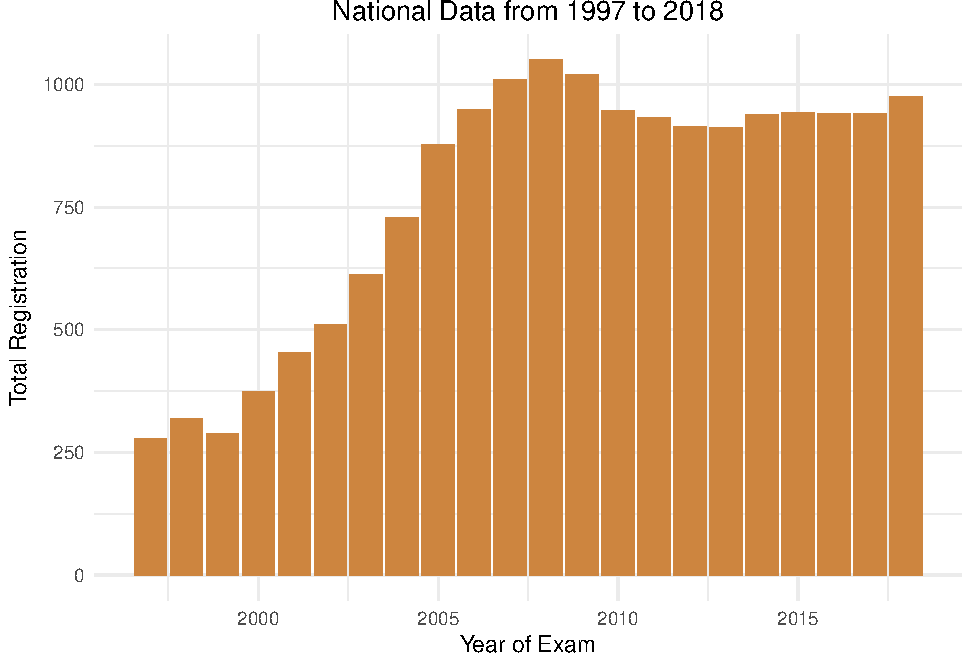
\includegraphics{NCEE_files/figure-latex/unnamed-chunk-2-1.pdf}

\begin{Shaded}
\begin{Highlighting}[]
\CommentTok{# =====Plot for National Data Trend===== #}

\NormalTok{population <-}\StringTok{ }\KeywordTok{c}\NormalTok{(national_JHS,national_reg)}
\NormalTok{label <-}\StringTok{ }\KeywordTok{c}\NormalTok{(}\KeywordTok{rep}\NormalTok{(}\StringTok{"JHS"}\NormalTok{,}\DecValTok{14}\NormalTok{),}\KeywordTok{rep}\NormalTok{(}\StringTok{"NCEE Reg"}\NormalTok{,}\DecValTok{14}\NormalTok{))}
\NormalTok{year_birth <-}\StringTok{ }\KeywordTok{rep}\NormalTok{(year_born,}\DecValTok{2}\NormalTok{)}
\NormalTok{plot_df <-}\StringTok{ }\KeywordTok{data.frame}\NormalTok{(population,label,year_birth)}

\NormalTok{p1 <-}\StringTok{ }\KeywordTok{ggplot}\NormalTok{(}\DataTypeTok{data=}\NormalTok{plot_df, }\KeywordTok{aes}\NormalTok{(}\DataTypeTok{x=}\NormalTok{year_birth, }\DataTypeTok{y=}\NormalTok{ population, }\DataTypeTok{fill=}\NormalTok{label)) }\OperatorTok{+}
\KeywordTok{geom_bar}\NormalTok{(}\DataTypeTok{stat=}\StringTok{"identity"}\NormalTok{, }\DataTypeTok{color=}\StringTok{"grey"}\NormalTok{, }\DataTypeTok{position=}\KeywordTok{position_dodge}\NormalTok{()) }\OperatorTok{+}
\StringTok{  }\KeywordTok{theme_minimal}\NormalTok{() }\OperatorTok{+}
\StringTok{  }\KeywordTok{scale_fill_brewer}\NormalTok{(}\DataTypeTok{palette=}\StringTok{"Blues"}\NormalTok{) }\OperatorTok{+}
\StringTok{  }\KeywordTok{ggtitle}\NormalTok{(}\StringTok{"Total-Cohort from 1987 to 2000"}\NormalTok{) }\OperatorTok{+}
\StringTok{  }\KeywordTok{theme}\NormalTok{(}\DataTypeTok{plot.title =} \KeywordTok{element_text}\NormalTok{(}\DataTypeTok{hjust =} \FloatTok{0.5}\NormalTok{)) }\OperatorTok{+}
\StringTok{  }\KeywordTok{xlab}\NormalTok{(}\StringTok{"Year of Birth"}\NormalTok{)}

\CommentTok{# =====Plot for Beijing Data Trend===== #}

\NormalTok{Beijing_JHS <-}\StringTok{ }\KeywordTok{as.numeric}\NormalTok{(NCEE_JHS[}\DecValTok{1}\NormalTok{,}\DecValTok{7}\OperatorTok{:}\DecValTok{19}\NormalTok{])}\OperatorTok{/}\DecValTok{30000}  \CommentTok{#2012-2000}
\NormalTok{Beijing_reg <-}\StringTok{ }\KeywordTok{as.numeric}\NormalTok{(NCEE_reg[}\DecValTok{1}\NormalTok{,}\DecValTok{1}\OperatorTok{:}\DecValTok{13}\NormalTok{])}\OperatorTok{/}\DecValTok{10000} \CommentTok{# 2018-2006}
\NormalTok{label_city <-}\StringTok{ }\KeywordTok{c}\NormalTok{(}\KeywordTok{rep}\NormalTok{(}\StringTok{"JHS"}\NormalTok{,}\DecValTok{13}\NormalTok{),}\KeywordTok{rep}\NormalTok{(}\StringTok{"NCEE Reg"}\NormalTok{,}\DecValTok{13}\NormalTok{))}
\NormalTok{year_born <-}\StringTok{ }\KeywordTok{c}\NormalTok{(}\DecValTok{2000}\OperatorTok{:}\DecValTok{1988}\NormalTok{)}
\NormalTok{year_birth <-}\StringTok{ }\KeywordTok{rep}\NormalTok{(year_born,}\DecValTok{2}\NormalTok{)}
\NormalTok{Beijing_population <-}\StringTok{ }\KeywordTok{c}\NormalTok{(Beijing_JHS,Beijing_reg)}
\NormalTok{plot_beijing <-}\StringTok{ }\KeywordTok{data.frame}\NormalTok{(Beijing_population,label_city,year_birth)}

\NormalTok{p2 <-}\StringTok{ }\KeywordTok{ggplot}\NormalTok{(}\DataTypeTok{data=}\NormalTok{plot_beijing, }\KeywordTok{aes}\NormalTok{(}\DataTypeTok{x=}\NormalTok{year_birth, }\DataTypeTok{y=}\NormalTok{ Beijing_population, }\DataTypeTok{fill=}\NormalTok{label_city)) }\OperatorTok{+}
\KeywordTok{geom_bar}\NormalTok{(}\DataTypeTok{stat=}\StringTok{"identity"}\NormalTok{, }\DataTypeTok{color=}\StringTok{"grey"}\NormalTok{, }\DataTypeTok{position=}\KeywordTok{position_dodge}\NormalTok{()) }\OperatorTok{+}
\StringTok{  }\KeywordTok{theme_minimal}\NormalTok{() }\OperatorTok{+}
\StringTok{  }\KeywordTok{scale_fill_brewer}\NormalTok{(}\DataTypeTok{palette=}\StringTok{"Reds"}\NormalTok{) }\OperatorTok{+}
\StringTok{  }\KeywordTok{ggtitle}\NormalTok{(}\StringTok{"Beijing-Cohort from 1987 to 2000"}\NormalTok{) }\OperatorTok{+}
\StringTok{  }\KeywordTok{theme}\NormalTok{(}\DataTypeTok{plot.title =} \KeywordTok{element_text}\NormalTok{(}\DataTypeTok{hjust =} \FloatTok{0.5}\NormalTok{)) }\OperatorTok{+}
\StringTok{  }\KeywordTok{xlab}\NormalTok{(}\StringTok{"Year of Birth"}\NormalTok{)}

\CommentTok{# =====Plot for Henan Data Trend===== #}

\NormalTok{Henan_JHS <-}\StringTok{ }\KeywordTok{as.numeric}\NormalTok{(NCEE_JHS[}\DecValTok{16}\NormalTok{,}\DecValTok{7}\OperatorTok{:}\DecValTok{19}\NormalTok{])}\OperatorTok{/}\DecValTok{30000}  \CommentTok{#2012-2000}
\NormalTok{Henan_reg <-}\StringTok{ }\KeywordTok{as.numeric}\NormalTok{(NCEE_reg[}\DecValTok{16}\NormalTok{,}\DecValTok{1}\OperatorTok{:}\DecValTok{13}\NormalTok{])}\OperatorTok{/}\DecValTok{10000} \CommentTok{# 2018-2006}
\NormalTok{label_city <-}\StringTok{ }\KeywordTok{c}\NormalTok{(}\KeywordTok{rep}\NormalTok{(}\StringTok{"JHS"}\NormalTok{,}\DecValTok{13}\NormalTok{),}\KeywordTok{rep}\NormalTok{(}\StringTok{"NCEE Reg"}\NormalTok{,}\DecValTok{13}\NormalTok{))}
\NormalTok{year_born <-}\StringTok{ }\KeywordTok{c}\NormalTok{(}\DecValTok{2000}\OperatorTok{:}\DecValTok{1988}\NormalTok{)}
\NormalTok{year_birth <-}\StringTok{ }\KeywordTok{rep}\NormalTok{(year_born,}\DecValTok{2}\NormalTok{)}
\NormalTok{Henan_population <-}\StringTok{ }\KeywordTok{c}\NormalTok{(Henan_JHS,Henan_reg)}
\NormalTok{plot_Henan <-}\StringTok{ }\KeywordTok{data.frame}\NormalTok{(Henan_population,label_city,year_birth)}

\NormalTok{p3 <-}\StringTok{ }\KeywordTok{ggplot}\NormalTok{(}\DataTypeTok{data=}\NormalTok{plot_Henan, }\KeywordTok{aes}\NormalTok{(}\DataTypeTok{x=}\NormalTok{year_birth, }\DataTypeTok{y=}\NormalTok{ Henan_population, }\DataTypeTok{fill=}\NormalTok{label_city)) }\OperatorTok{+}
\KeywordTok{geom_bar}\NormalTok{(}\DataTypeTok{stat=}\StringTok{"identity"}\NormalTok{, }\DataTypeTok{color=}\StringTok{"grey"}\NormalTok{, }\DataTypeTok{position=}\KeywordTok{position_dodge}\NormalTok{()) }\OperatorTok{+}
\StringTok{  }\KeywordTok{theme_minimal}\NormalTok{() }\OperatorTok{+}
\StringTok{  }\KeywordTok{scale_fill_brewer}\NormalTok{(}\DataTypeTok{palette=}\StringTok{"Greens"}\NormalTok{) }\OperatorTok{+}
\StringTok{  }\KeywordTok{ggtitle}\NormalTok{(}\StringTok{"Henan-Cohort from 1987 to 2000"}\NormalTok{) }\OperatorTok{+}
\StringTok{  }\KeywordTok{theme}\NormalTok{(}\DataTypeTok{plot.title =} \KeywordTok{element_text}\NormalTok{(}\DataTypeTok{hjust =} \FloatTok{0.5}\NormalTok{)) }\OperatorTok{+}
\StringTok{  }\KeywordTok{xlab}\NormalTok{(}\StringTok{"Year of Birth"}\NormalTok{)}

\CommentTok{# =====Plot for Shanxi Data Trend===== #}

\NormalTok{Xinjiang_JHS <-}\StringTok{ }\KeywordTok{as.numeric}\NormalTok{(NCEE_JHS[}\DecValTok{31}\NormalTok{,}\DecValTok{7}\OperatorTok{:}\DecValTok{19}\NormalTok{])}\OperatorTok{/}\DecValTok{30000}  \CommentTok{#2012-2000}
\NormalTok{Xinjiang_reg <-}\StringTok{ }\KeywordTok{as.numeric}\NormalTok{(NCEE_reg[}\DecValTok{31}\NormalTok{,}\DecValTok{1}\OperatorTok{:}\DecValTok{13}\NormalTok{])}\OperatorTok{/}\DecValTok{10000} \CommentTok{# 2018-2006}
\NormalTok{label_city <-}\StringTok{ }\KeywordTok{c}\NormalTok{(}\KeywordTok{rep}\NormalTok{(}\StringTok{"JHS"}\NormalTok{,}\DecValTok{13}\NormalTok{),}\KeywordTok{rep}\NormalTok{(}\StringTok{"NCEE Reg"}\NormalTok{,}\DecValTok{13}\NormalTok{))}
\NormalTok{year_born <-}\StringTok{ }\KeywordTok{c}\NormalTok{(}\DecValTok{2000}\OperatorTok{:}\DecValTok{1988}\NormalTok{)}
\NormalTok{year_birth <-}\StringTok{ }\KeywordTok{rep}\NormalTok{(year_born,}\DecValTok{2}\NormalTok{)}
\NormalTok{Xinjiang_population <-}\StringTok{ }\KeywordTok{c}\NormalTok{(Xinjiang_JHS,Xinjiang_reg)}
\NormalTok{plot_Xinjiang <-}\StringTok{ }\KeywordTok{data.frame}\NormalTok{(Xinjiang_population,label_city,year_birth)}

\NormalTok{p4 <-}\StringTok{ }\KeywordTok{ggplot}\NormalTok{(}\DataTypeTok{data=}\NormalTok{plot_Xinjiang, }\KeywordTok{aes}\NormalTok{(}\DataTypeTok{x=}\NormalTok{year_birth, }\DataTypeTok{y=}\NormalTok{ Xinjiang_population, }\DataTypeTok{fill=}\NormalTok{label_city)) }\OperatorTok{+}
\KeywordTok{geom_bar}\NormalTok{(}\DataTypeTok{stat=}\StringTok{"identity"}\NormalTok{, }\DataTypeTok{color=}\StringTok{"grey"}\NormalTok{, }\DataTypeTok{position=}\KeywordTok{position_dodge}\NormalTok{()) }\OperatorTok{+}
\StringTok{  }\KeywordTok{theme_minimal}\NormalTok{() }\OperatorTok{+}
\StringTok{  }\KeywordTok{scale_fill_brewer}\NormalTok{(}\DataTypeTok{palette=}\StringTok{"OrRd"}\NormalTok{) }\OperatorTok{+}
\StringTok{  }\KeywordTok{ggtitle}\NormalTok{(}\StringTok{"Xinjiang-Cohort from 1987 to 2000"}\NormalTok{) }\OperatorTok{+}
\StringTok{  }\KeywordTok{theme}\NormalTok{(}\DataTypeTok{plot.title =} \KeywordTok{element_text}\NormalTok{(}\DataTypeTok{hjust =} \FloatTok{0.5}\NormalTok{)) }\OperatorTok{+}
\StringTok{  }\KeywordTok{xlab}\NormalTok{(}\StringTok{"Year of Birth"}\NormalTok{)}

\CommentTok{# =====Display===== #}
\KeywordTok{grid.arrange}\NormalTok{(p1, p2, p3, p4, }\DataTypeTok{nrow =} \DecValTok{2}\NormalTok{)}
\end{Highlighting}
\end{Shaded}

\begin{verbatim}
## Warning: Removed 1 rows containing missing values (geom_bar).

## Warning: Removed 1 rows containing missing values (geom_bar).
\end{verbatim}

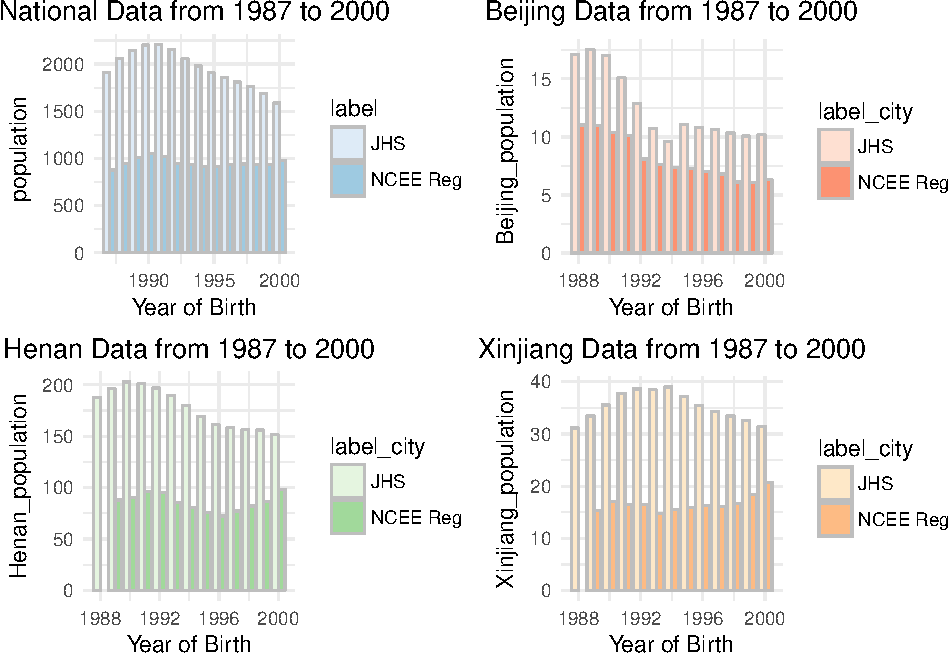
\includegraphics{NCEE_files/figure-latex/unnamed-chunk-3-1.pdf}

\begin{Shaded}
\begin{Highlighting}[]
\CommentTok{# =====Fit linear model for 31 provinces===== #}
\NormalTok{NCEE_function <-}\StringTok{ }\ControlFlowTok{function}\NormalTok{(JHS, reg)\{}
\NormalTok{  intercept <-}\StringTok{ }\KeywordTok{rep}\NormalTok{(}\OtherTok{NA}\NormalTok{, }\DecValTok{31}\NormalTok{)}
\NormalTok{  slope <-}\StringTok{ }\KeywordTok{rep}\NormalTok{(}\OtherTok{NA}\NormalTok{, }\DecValTok{31}\NormalTok{)}
\NormalTok{  cor <-}\StringTok{ }\KeywordTok{rep}\NormalTok{(}\OtherTok{NA}\NormalTok{,}\DecValTok{31}\NormalTok{)}
\NormalTok{  predict_year <-}\StringTok{ }\KeywordTok{c}\NormalTok{(}\StringTok{"2023"}\NormalTok{,}\StringTok{"2022"}\NormalTok{,}\StringTok{"2021"}\NormalTok{,}\StringTok{"2020"}\NormalTok{,}\StringTok{"2019"}\NormalTok{)}
\NormalTok{  prd_df <-}\StringTok{ }\KeywordTok{data.frame}\NormalTok{(predict_year)}
\NormalTok{  prd_low <-}\StringTok{ }\KeywordTok{data.frame}\NormalTok{(predict_year)}
\NormalTok{  prd_high <-}\StringTok{ }\KeywordTok{data.frame}\NormalTok{(predict_year)}
  
  \ControlFlowTok{for}\NormalTok{(i }\ControlFlowTok{in} \DecValTok{1}\OperatorTok{:}\DecValTok{31}\NormalTok{)\{}
\NormalTok{    city_JHS <-}\StringTok{ }\KeywordTok{as.numeric}\NormalTok{(JHS[i,}\DecValTok{7}\OperatorTok{:}\DecValTok{18}\NormalTok{])}\OperatorTok{/}\DecValTok{30000} \CommentTok{# 2012-2001}
\NormalTok{    city_reg <-}\StringTok{ }\KeywordTok{as.numeric}\NormalTok{(reg[i,}\DecValTok{1}\OperatorTok{:}\DecValTok{12}\NormalTok{])}\OperatorTok{/}\DecValTok{10000} \CommentTok{# 2018-2007}
\NormalTok{    city_lm.i <-}\StringTok{ }\KeywordTok{lm}\NormalTok{(city_reg}\OperatorTok{~}\NormalTok{city_JHS)}
    
\NormalTok{    intercept[i] <-}\StringTok{ }\KeywordTok{as.numeric}\NormalTok{(city_lm.i}\OperatorTok{$}\NormalTok{coefficients[}\DecValTok{1}\NormalTok{])}
\NormalTok{    slope[i] <-}\StringTok{ }\KeywordTok{as.numeric}\NormalTok{(city_lm.i}\OperatorTok{$}\NormalTok{coefficients[}\DecValTok{2}\NormalTok{])}
\NormalTok{    cor[i] <-}\StringTok{ }\KeywordTok{cor}\NormalTok{(city_JHS,city_reg)}
    
\NormalTok{    predict_city <-}\KeywordTok{predict}\NormalTok{(city_lm.i,}\DataTypeTok{newdata=}\KeywordTok{data.frame}\NormalTok{(}\DataTypeTok{city_JHS=}\KeywordTok{as.numeric}\NormalTok{(NCEE_JHS[i,}\DecValTok{2}\OperatorTok{:}\DecValTok{6}\NormalTok{])}\OperatorTok{/}\DecValTok{30000}\NormalTok{))}
\NormalTok{    predict_city_low <-}\KeywordTok{predict}\NormalTok{(city_lm.i,}\DataTypeTok{newdata=}\KeywordTok{data.frame}\NormalTok{(}\DataTypeTok{city_JHS=}\KeywordTok{as.numeric}\NormalTok{(NCEE_JHS[i,}\DecValTok{2}\OperatorTok{:}\DecValTok{6}\NormalTok{])}\OperatorTok{/}\DecValTok{30000}\NormalTok{), }\DataTypeTok{interval =} \StringTok{"confidence"}\NormalTok{)[,}\DecValTok{2}\NormalTok{]}
\NormalTok{    predict_city_high <-}\KeywordTok{predict}\NormalTok{(city_lm.i,}\DataTypeTok{newdata=}\KeywordTok{data.frame}\NormalTok{(}\DataTypeTok{city_JHS=}\KeywordTok{as.numeric}\NormalTok{(NCEE_JHS[i,}\DecValTok{2}\OperatorTok{:}\DecValTok{6}\NormalTok{])}\OperatorTok{/}\DecValTok{30000}\NormalTok{), }\DataTypeTok{interval =} \StringTok{"confidence"}\NormalTok{)[,}\DecValTok{3}\NormalTok{]}
    
\NormalTok{    prd_df <-}\StringTok{ }\KeywordTok{data.frame}\NormalTok{(prd_df, predict_city)}
\NormalTok{    prd_low <-}\StringTok{ }\KeywordTok{data.frame}\NormalTok{(prd_low, predict_city_low)}
\NormalTok{    prd_high <-}\StringTok{ }\KeywordTok{data.frame}\NormalTok{(prd_high, predict_city_high)}
    
\NormalTok{  \}}
  
  \KeywordTok{colnames}\NormalTok{(prd_df) <-}\StringTok{ }\KeywordTok{c}\NormalTok{(}\StringTok{"year"}\NormalTok{, province)}
  \KeywordTok{colnames}\NormalTok{(prd_low) <-}\StringTok{ }\KeywordTok{c}\NormalTok{(}\StringTok{"year"}\NormalTok{, province)}
  \KeywordTok{colnames}\NormalTok{(prd_high) <-}\StringTok{ }\KeywordTok{c}\NormalTok{(}\StringTok{"year"}\NormalTok{, province)}
  
\NormalTok{  summ <-}\StringTok{ }\KeywordTok{data.frame}\NormalTok{(province,intercept,slope,cor)}
  
  \KeywordTok{return}\NormalTok{(}\KeywordTok{list}\NormalTok{(summ, prd_df,prd_low,prd_high))}
\NormalTok{\}}

\KeywordTok{NCEE_function}\NormalTok{(NCEE_JHS,NCEE_reg)}
\end{Highlighting}
\end{Shaded}

\begin{verbatim}
## [[1]]
##        province    intercept       slope         cor
## 1       Beijing   0.74159366  0.58367386  0.95796677
## 2       Tianjin   1.67394522  0.44272559  0.94405284
## 3         Hebei  29.62146866  0.17103556  0.84485710
## 4        Shanxi   9.08394803  0.42714380  0.88286680
## 5     Neimenggu   6.94530803  0.44748932  0.78112423
## 6      Liaoning   6.29141297  0.35801846  0.96672856
## 7         Jilin   5.56139524  0.33929183  0.88834426
## 8  Heilongjiang  14.00399733  0.12099640  0.81848106
## 9      Shanghai -12.91471720  1.26550835  0.87726284
## 10      Jiangsu   7.20393799  0.38086228  0.97929885
## 11     Zhejiang  10.21780369  0.36660930  0.83230778
## 12        Anhui  39.49320895  0.13759774  0.54835237
## 13       Fujian  -0.06537096  0.47495530  0.92248816
## 14      Jiangxi  10.14888553  0.35215698  0.56782546
## 15     Shandong  25.70346635  0.27652718  0.97186677
## 16        Henan  54.43992172  0.17707451  0.41904289
## 17        Hubei  16.22275744  0.30671198  0.90604763
## 18        Hunan  25.50320882  0.18716064  0.72314704
## 19    Guangdong -10.15613797  0.51255036  0.81123954
## 20      Guangxi  61.67693726 -0.40297177 -0.72825130
## 21       Hainan   3.41220865  0.15224077  0.36042056
## 22    Chongqing  23.46688139 -0.02478205 -0.02015415
## 23      Sichuan 108.07795856 -0.45671917 -0.76100780
## 24      Guizhou -28.99491535  0.87234873  0.58919244
## 25       Yunnan -23.81550933  0.75106341  0.69658345
## 26       Xizang   0.81776576  0.30723486  0.71501871
## 27      Shaanxi  17.15826286  0.30423227  0.86844271
## 28        Gansu  17.29251111  0.26128669  0.81578300
## 29      Qinghai   2.26442204  0.25589734  0.35055141
## 30      Ningxia  -2.20551474  0.89213892  0.88858472
## 31     Xinjiang  31.25825654 -0.41123584 -0.67414089
## 
## [[2]]
##   year  Beijing  Tianjin    Hebei   Shanxi Neimenggu Liaoning    Jilin
## 1 2023 5.924695 5.544001 44.44840 24.49572  16.17336 17.78918 12.55877
## 2 2022 5.961058 5.457522 43.51417 24.64250  16.07970 17.96637 12.39560
## 3 2021 6.254705 5.532653 43.08385 25.12817  16.48650 18.37983 12.29654
## 4 2020 6.710418 5.617361 42.66689 26.43954  16.93412 18.88962 12.60603
## 5 2019 6.783941 5.521378 41.52822 27.47166  17.21465 18.91142 12.85609
##   Heilongjiang Shanghai  Jiangsu Zhejiang    Anhui   Fujian  Jiangxi
## 1     17.64995 4.452782 33.69842 29.26267 48.76559 19.18167 32.57449
## 2     17.64955 4.519685 31.95308 28.59859 48.40031 18.21658 31.30272
## 3     17.63309 4.479484 30.90837 28.29596 48.21134 17.87936 30.85554
## 4     17.69960 5.088784 30.71620 28.53681 48.31843 17.75699 30.69235
## 5     17.76634 5.506697 30.78527 28.33623 48.65305 17.47989 30.74257
##   Shandong    Henan    Hubei    Hunan Guangdong  Guangxi   Hainan
## 1 56.07169 79.77112 31.42679 39.82907  50.68361 34.34696 5.103817
## 2 54.82297 78.98405 30.68795 39.60641  49.27305 34.97952 5.055069
## 3 54.35285 78.33378 30.18141 39.37891  50.54981 35.30832 5.081219
## 4 54.71996 78.01212 30.29000 39.26790  54.21173 35.47244 5.124156
## 5 55.01350 77.16739 31.39181 38.87176  59.00239 35.47355 5.172061
##   Chongqing  Sichuan  Guizhou   Yunnan   Xizang  Shaanxi    Gansu  Qinghai
## 1  22.64874 70.14950 24.21458 23.07108 2.093518 27.80288 24.74900 4.019997
## 2  22.66888 70.80611 26.00408 23.07964 2.049603 27.81690 24.92357 4.038106
## 3  22.67354 70.56822 28.57135 23.60869 2.021307 28.01711 25.21172 4.082701
## 4  22.65784 68.74964 31.14847 23.70092 2.090691 28.48872 25.74878 4.072704
## 5  22.62628 66.71141 32.15769 23.11138 2.109350 29.34632 26.31509 4.039454
##    Ningxia Xinjiang
## 1 6.096730 18.89643
## 2 5.933647 18.99249
## 3 5.952590 18.81974
## 4 6.071245 18.76386
## 5 6.262608 18.66796
## 
## [[3]]
##   year  Beijing  Tianjin    Hebei   Shanxi Neimenggu Liaoning    Jilin
## 1 2023 5.401446 5.153520 41.78669 20.68401  13.15938 16.45014 10.89727
## 2 2022 5.443723 5.050594 40.58436 20.88497  13.01673 16.65751 10.68037
## 3 2021 5.783270 5.140039 40.01933 21.54969  13.63531 17.14081 10.54850
## 4 2020 6.301734 5.240451 39.46628 23.34282  14.31260 17.73543 10.96003
## 5 2019 6.384136 5.126638 37.93307 24.75166  14.73485 17.76083 11.29146
##   Heilongjiang Shanghai  Jiangsu Zhejiang    Anhui   Fujian  Jiangxi
## 1     16.08810 3.359065 31.75634 27.71617 43.24645 16.99420 29.94066
## 2     16.08751 3.445027 29.79474 26.79009 42.51294 15.79660 27.88378
## 3     16.06371 3.393407 28.61686 26.36316 42.13228 15.37560 27.09229
## 4     16.15987 4.162961 28.39994 26.70314 42.34809 15.22256 26.79769
## 5     16.25623 4.670148 28.47791 26.42012 43.02082 14.87546 26.88864
##   Shandong    Henan    Hubei    Hunan Guangdong  Guangxi   Hainan
## 1 54.31400 69.32896 26.87926 36.39080  41.06704 31.92888 4.161633
## 2 52.91811 67.48216 25.91698 36.08266  38.96843 32.24008 4.029560
## 3 52.38944 65.93681 25.25619 35.76350  40.86816 32.39198 4.100530
## 4 52.80241 65.16707 25.39791 35.60627  46.29413 32.46578 4.216426
## 5 53.13192 63.13196 26.83375 35.03786  53.30004 32.46628 4.344581
##   Chongqing  Sichuan  Guizhou   Yunnan   Xizang  Shaanxi    Gansu  Qinghai
## 1  14.60237 60.66254 17.73032 21.01130 1.891626 24.06460 22.63066 3.798383
## 2  13.93724 60.93050 20.72582 21.02361 1.853635 24.08398 22.89095 3.835638
## 3  13.78302 60.83347 24.33437 21.75810 1.826744 24.36074 23.32026 3.906896
## 4  14.30221 60.08953 26.63361 21.88022 1.889312 25.01192 24.11915 3.893978
## 5  15.33986 59.24962 27.18621 21.06913 1.904268 26.19303 24.95880 3.838253
##    Ningxia Xinjiang
## 1 5.928326 16.96881
## 2 5.738951 16.99696
## 3 5.761707 16.94600
## 4 5.899816 16.92916
## 5 6.101769 16.89984
## 
## [[4]]
##   year  Beijing  Tianjin    Hebei   Shanxi Neimenggu Liaoning    Jilin
## 1 2023 6.447945 5.934483 47.11011 28.30743  19.18734 19.12822 14.22027
## 2 2022 6.478393 5.864451 46.44399 28.40004  19.14266 19.27524 14.11084
## 3 2021 6.726139 5.925266 46.14837 28.70665  19.33768 19.61886 14.04458
## 4 2020 7.119101 5.994271 45.86751 29.53626  19.55564 20.04380 14.25204
## 5 2019 7.183746 5.916118 45.12338 30.19167  19.69446 20.06201 14.42072
##   Heilongjiang Shanghai  Jiangsu Zhejiang    Anhui   Fujian  Jiangxi
## 1     19.21181 5.546499 35.64050 30.80916 54.28472 21.36914 35.20832
## 2     19.21159 5.594343 34.11142 30.40709 54.28767 20.63656 34.72166
## 3     19.20248 5.565561 33.19989 30.22875 54.29040 20.38312 34.61879
## 4     19.23933 6.014607 33.03247 30.37047 54.28876 20.29143 34.58701
## 5     19.27645 6.343246 33.09263 30.25234 54.28528 20.08431 34.59650
##   Shandong    Henan    Hubei    Hunan Guangdong  Guangxi   Hainan
## 1 57.82938 90.21329 35.97432 43.26734  60.30017 36.76505 6.046001
## 2 56.72782 90.48595 35.45891 43.13016  59.57767 37.71896 6.080579
## 3 56.31626 90.73076 35.10664 42.99432  60.23147 38.22466 6.061908
## 4 56.63751 90.85716 35.18209 42.92953  62.12933 38.47909 6.031886
## 5 56.89509 91.20283 35.94988 42.70566  64.70473 38.48082 5.999542
##   Chongqing  Sichuan  Guizhou   Yunnan   Xizang  Shaanxi    Gansu  Qinghai
## 1  30.69512 79.63646 30.69884 25.13085 2.295409 31.54116 26.86733 4.241611
## 2  31.40053 80.68172 31.28234 25.13567 2.245572 31.54981 26.95620 4.240574
## 3  31.56406 80.30297 32.80833 25.45928 2.215870 31.67349 27.10318 4.258505
## 4  31.01347 77.40975 35.66333 25.52162 2.292070 31.96552 27.37842 4.251429
## 5  29.91270 74.17320 37.12917 25.15363 2.314433 32.49962 27.67138 4.240655
##    Ningxia Xinjiang
## 1 6.265134 20.82404
## 2 6.128343 20.98802
## 3 6.143473 20.69349
## 4 6.242674 20.59855
## 5 6.423447 20.43608
\end{verbatim}

\begin{Shaded}
\begin{Highlighting}[]
\NormalTok{path <-}\StringTok{ }\KeywordTok{file.path}\NormalTok{(wd,}\StringTok{"output"}\NormalTok{)}

\KeywordTok{write.csv}\NormalTok{(}\KeywordTok{NCEE_function}\NormalTok{(NCEE_JHS,NCEE_reg)[[}\DecValTok{2}\NormalTok{]], }\KeywordTok{file.path}\NormalTok{(path, }\StringTok{"province prediction_fit.csv"}\NormalTok{))}
\KeywordTok{write.csv}\NormalTok{(}\KeywordTok{NCEE_function}\NormalTok{(NCEE_JHS,NCEE_reg)[[}\DecValTok{3}\NormalTok{]], }\KeywordTok{file.path}\NormalTok{(path, }\StringTok{"province prediction_low.csv"}\NormalTok{))}
\KeywordTok{write.csv}\NormalTok{(}\KeywordTok{NCEE_function}\NormalTok{(NCEE_JHS,NCEE_reg)[[}\DecValTok{4}\NormalTok{]], }\KeywordTok{file.path}\NormalTok{(path, }\StringTok{"province prediction_high.csv"}\NormalTok{))}

\CommentTok{# Sum up all province prediction as the national total}
\NormalTok{predict_national <-}\StringTok{ }\KeywordTok{rep}\NormalTok{(}\OtherTok{NA}\NormalTok{,}\DecValTok{5}\NormalTok{)}
\ControlFlowTok{for}\NormalTok{ (i }\ControlFlowTok{in} \DecValTok{1}\OperatorTok{:}\DecValTok{5}\NormalTok{) \{}
\NormalTok{  predict_national[i] <-}\StringTok{ }\KeywordTok{sum}\NormalTok{(}\KeywordTok{as.numeric}\NormalTok{(}\KeywordTok{NCEE_function}\NormalTok{(NCEE_JHS,NCEE_reg)[[}\DecValTok{2}\NormalTok{]][i,]))}
\NormalTok{\} }\CommentTok{# 2023-2019}
\end{Highlighting}
\end{Shaded}

\begin{Shaded}
\begin{Highlighting}[]
\CommentTok{# =====Use National JHS as Predictors===== #}

\NormalTok{JHS_total <-}\StringTok{ }\NormalTok{NCEE_national}\OperatorTok{$}\NormalTok{JHS[}\DecValTok{7}\OperatorTok{:}\DecValTok{17}\NormalTok{]}\OperatorTok{/}\DecValTok{30000}
\NormalTok{Reg_total <-}\StringTok{ }\NormalTok{NCEE_national}\OperatorTok{$}\NormalTok{Reg[}\DecValTok{1}\OperatorTok{:}\DecValTok{11}\NormalTok{]}
\NormalTok{new.data <-}\StringTok{  }\NormalTok{NCEE_national}\OperatorTok{$}\NormalTok{JHS[}\DecValTok{2}\OperatorTok{:}\DecValTok{6}\NormalTok{]}\OperatorTok{/}\DecValTok{30000}

\NormalTok{test <-}\StringTok{ }\KeywordTok{data.frame}\NormalTok{(JHS_total, Reg_total)}

\NormalTok{predict_national2 <-}\StringTok{ }\KeywordTok{predict}\NormalTok{(}\KeywordTok{lm}\NormalTok{(Reg_total}\OperatorTok{~}\NormalTok{JHS_total, }\DataTypeTok{data =}\NormalTok{ test),}\DataTypeTok{newdata=}\KeywordTok{data.frame}\NormalTok{(}\DataTypeTok{JHS_total=}\NormalTok{new.data), }\DataTypeTok{interval =} \StringTok{"confidence"}\NormalTok{) }
\NormalTok{predict_national;predict_national2}
\end{Highlighting}
\end{Shaded}

\begin{verbatim}
## [1] 838.4952 830.3795 831.1387 839.2643 843.9974
\end{verbatim}

\begin{verbatim}
##        fit      lwr      upr
## 1 915.4487 847.6075 983.2899
## 2 912.1054 839.5374 984.6734
## 3 911.5534 838.1994 984.9074
## 4 910.7361 836.2158 985.2563
## 5 915.0885 846.7411 983.4360
\end{verbatim}

\begin{Shaded}
\begin{Highlighting}[]
\CommentTok{# =====Plot prediction result===== #}

\NormalTok{national_reg <-}\StringTok{ }\KeywordTok{c}\NormalTok{(}\KeywordTok{rep}\NormalTok{(}\DecValTok{0}\NormalTok{,}\DecValTok{5}\NormalTok{),NCEE_national}\OperatorTok{$}\NormalTok{Reg[}\DecValTok{1}\OperatorTok{:}\DecValTok{14}\NormalTok{])}
\NormalTok{national_JHS <-}\StringTok{ }\NormalTok{NCEE_national}\OperatorTok{$}\NormalTok{JHS[}\DecValTok{2}\OperatorTok{:}\DecValTok{20}\NormalTok{]}\OperatorTok{/}\DecValTok{30000}
\NormalTok{year_born <-}\StringTok{ }\KeywordTok{c}\NormalTok{(}\DecValTok{2005}\OperatorTok{:}\DecValTok{1987}\NormalTok{)}
\NormalTok{predict_national_t <-}\StringTok{ }\KeywordTok{c}\NormalTok{(}\KeywordTok{rep}\NormalTok{(}\OtherTok{NA}\NormalTok{,}\DecValTok{19}\NormalTok{),predict_national,national_reg[}\DecValTok{6}\OperatorTok{:}\DecValTok{19}\NormalTok{])}

\NormalTok{predict_national_pf <-}\StringTok{ }\KeywordTok{c}\NormalTok{(}\KeywordTok{rep}\NormalTok{(}\OtherTok{NA}\NormalTok{,}\DecValTok{19}\NormalTok{),prd_fit <-}\StringTok{ }\NormalTok{predict_national2[,}\DecValTok{1}\NormalTok{],national_reg[}\DecValTok{6}\OperatorTok{:}\DecValTok{19}\NormalTok{])}
\NormalTok{predict_national_pl <-}\StringTok{ }\KeywordTok{c}\NormalTok{(}\KeywordTok{rep}\NormalTok{(}\OtherTok{NA}\NormalTok{,}\DecValTok{19}\NormalTok{),prd_fit <-}\StringTok{ }\NormalTok{predict_national2[,}\DecValTok{2}\NormalTok{],}\KeywordTok{rep}\NormalTok{(}\OtherTok{NA}\NormalTok{,}\DecValTok{14}\NormalTok{))}
\NormalTok{predict_national_ph <-}\StringTok{ }\KeywordTok{c}\NormalTok{(}\KeywordTok{rep}\NormalTok{(}\OtherTok{NA}\NormalTok{,}\DecValTok{19}\NormalTok{),prd_fit <-}\StringTok{ }\NormalTok{predict_national2[,}\DecValTok{3}\NormalTok{],}\KeywordTok{rep}\NormalTok{(}\OtherTok{NA}\NormalTok{,}\DecValTok{14}\NormalTok{))}

\NormalTok{population <-}\StringTok{ }\KeywordTok{c}\NormalTok{(national_JHS,national_reg)}
\NormalTok{label <-}\StringTok{ }\KeywordTok{c}\NormalTok{(}\KeywordTok{rep}\NormalTok{(}\StringTok{"JHS"}\NormalTok{,}\DecValTok{19}\NormalTok{),}\KeywordTok{rep}\NormalTok{(}\StringTok{"NCEE Reg"}\NormalTok{,}\DecValTok{19}\NormalTok{))}
\NormalTok{year_birth <-}\StringTok{ }\KeywordTok{rep}\NormalTok{(year_born,}\DecValTok{2}\NormalTok{)}

\NormalTok{plot_df <-}\StringTok{ }\KeywordTok{data.frame}\NormalTok{(population,label,year_birth,predict_national_t,predict_national_pf,predict_national_pl,predict_national_ph)}

\KeywordTok{ggplot}\NormalTok{(}\DataTypeTok{data=}\NormalTok{plot_df, }\KeywordTok{aes}\NormalTok{(}\DataTypeTok{x=}\NormalTok{year_birth, }\DataTypeTok{y=}\NormalTok{ population, }\DataTypeTok{fill=}\NormalTok{label)) }\OperatorTok{+}
\StringTok{  }\KeywordTok{geom_bar}\NormalTok{(}\DataTypeTok{stat=}\StringTok{"identity"}\NormalTok{, }\DataTypeTok{color=}\StringTok{"grey"}\NormalTok{, }\DataTypeTok{position=}\KeywordTok{position_dodge}\NormalTok{()) }\OperatorTok{+}
\StringTok{  }\KeywordTok{geom_point}\NormalTok{(}\KeywordTok{aes}\NormalTok{(}\DataTypeTok{x=}\NormalTok{year_birth, }\DataTypeTok{y=}\NormalTok{predict_national_pf),}\DataTypeTok{color=}\StringTok{'cornflowerblue'}\NormalTok{,}\DataTypeTok{shape=}\DecValTok{17}\NormalTok{) }\OperatorTok{+}
\StringTok{  }\KeywordTok{geom_point}\NormalTok{(}\KeywordTok{aes}\NormalTok{(}\DataTypeTok{x=}\NormalTok{year_birth, }\DataTypeTok{y=}\NormalTok{predict_national_t)) }\OperatorTok{+}
\StringTok{  }\KeywordTok{geom_line}\NormalTok{(}\KeywordTok{aes}\NormalTok{(}\DataTypeTok{x=}\NormalTok{year_birth, }\DataTypeTok{y=}\NormalTok{predict_national_pf),}\DataTypeTok{linetype=}\StringTok{"dotted"}\NormalTok{) }\OperatorTok{+}
\StringTok{  }\KeywordTok{geom_line}\NormalTok{(}\KeywordTok{aes}\NormalTok{(}\DataTypeTok{x=}\NormalTok{year_birth, }\DataTypeTok{y=}\NormalTok{predict_national_t),}\DataTypeTok{linetype=}\StringTok{"dotted"}\NormalTok{) }\OperatorTok{+}
\StringTok{  }\KeywordTok{geom_ribbon}\NormalTok{(}\KeywordTok{aes}\NormalTok{(}\DataTypeTok{ymin=}\NormalTok{predict_national_pl, }\DataTypeTok{ymax=}\NormalTok{predict_national_ph,}\DataTypeTok{x=}\NormalTok{year_birth), }\DataTypeTok{linetype=}\DecValTok{2}\NormalTok{, }\DataTypeTok{alpha=}\FloatTok{0.4}\NormalTok{) }\OperatorTok{+}
\StringTok{    }\KeywordTok{theme_minimal}\NormalTok{() }\OperatorTok{+}
\StringTok{    }\KeywordTok{scale_fill_brewer}\NormalTok{(}\DataTypeTok{palette=}\StringTok{"Blues"}\NormalTok{) }\OperatorTok{+}
\StringTok{    }\KeywordTok{ggtitle}\NormalTok{(}\StringTok{"National Data from Cohort 1987 to 2000 and Prediction"}\NormalTok{) }\OperatorTok{+}
\StringTok{    }\KeywordTok{theme}\NormalTok{(}\DataTypeTok{plot.title =} \KeywordTok{element_text}\NormalTok{(}\DataTypeTok{hjust =} \FloatTok{0.5}\NormalTok{)) }\OperatorTok{+}
\StringTok{    }\KeywordTok{xlab}\NormalTok{(}\StringTok{"Year of Birth"}\NormalTok{)}
\end{Highlighting}
\end{Shaded}

\begin{verbatim}
## Warning: Removed 19 rows containing missing values (geom_point).

## Warning: Removed 19 rows containing missing values (geom_point).
\end{verbatim}

\begin{verbatim}
## Warning: Removed 19 rows containing missing values (geom_path).

## Warning: Removed 19 rows containing missing values (geom_path).
\end{verbatim}

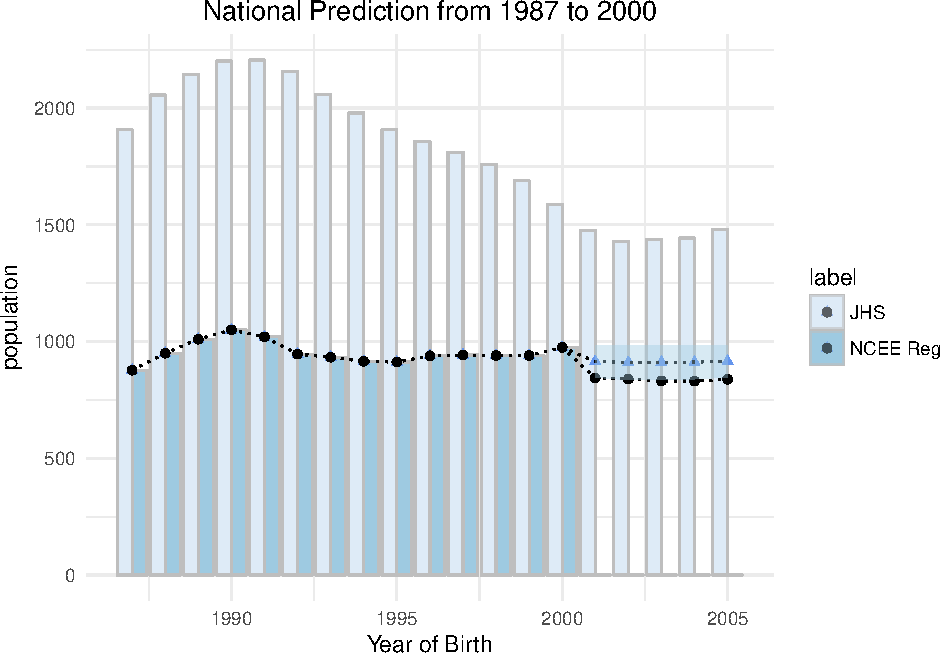
\includegraphics{NCEE_files/figure-latex/unnamed-chunk-6-1.pdf}

\begin{Shaded}
\begin{Highlighting}[]
\NormalTok{new_born <-}\StringTok{ }\KeywordTok{c}\NormalTok{(}\DecValTok{2005}\OperatorTok{:}\DecValTok{2001}\NormalTok{)}
\NormalTok{new_plot <-}\StringTok{ }\KeywordTok{data.frame}\NormalTok{(new_born,predict_national,predict_national2[,}\DecValTok{1}\NormalTok{],predict_national2[,}\DecValTok{2}\NormalTok{],predict_national2[,}\DecValTok{3}\NormalTok{])}

\KeywordTok{ggplot}\NormalTok{(}\DataTypeTok{data=}\NormalTok{new_plot) }\OperatorTok{+}
\StringTok{  }\KeywordTok{geom_line}\NormalTok{(}\KeywordTok{aes}\NormalTok{(}\DataTypeTok{x=}\NormalTok{new_born, }\DataTypeTok{y=}\NormalTok{predict_national2[,}\DecValTok{1}\NormalTok{]),}\DataTypeTok{linetype=}\StringTok{"dotted"}\NormalTok{,}\DataTypeTok{color=}\StringTok{'cornflowerblue'}\NormalTok{) }\OperatorTok{+}
\StringTok{  }\KeywordTok{geom_line}\NormalTok{(}\KeywordTok{aes}\NormalTok{(}\DataTypeTok{x=}\NormalTok{new_born, }\DataTypeTok{y=}\NormalTok{predict_national),}\DataTypeTok{linetype=}\StringTok{"dotted"}\NormalTok{) }\OperatorTok{+}
\StringTok{  }\KeywordTok{geom_point}\NormalTok{(}\KeywordTok{aes}\NormalTok{(}\DataTypeTok{x=}\NormalTok{new_born, }\DataTypeTok{y=}\NormalTok{predict_national2[,}\DecValTok{1}\NormalTok{]),}\DataTypeTok{color=}\StringTok{'cornflowerblue'}\NormalTok{,}\DataTypeTok{shape=}\DecValTok{17}\NormalTok{, }\DataTypeTok{size=}\DecValTok{3}\NormalTok{) }\OperatorTok{+}
\StringTok{  }\KeywordTok{geom_point}\NormalTok{(}\KeywordTok{aes}\NormalTok{(}\DataTypeTok{x=}\NormalTok{new_born, }\DataTypeTok{y=}\NormalTok{predict_national), }\DataTypeTok{size=}\DecValTok{3}\NormalTok{) }\OperatorTok{+}
\StringTok{  }\KeywordTok{geom_ribbon}\NormalTok{(}\KeywordTok{aes}\NormalTok{(}\DataTypeTok{ymin=}\NormalTok{predict_national2[,}\DecValTok{2}\NormalTok{], }\DataTypeTok{ymax=}\NormalTok{predict_national2[,}\DecValTok{3}\NormalTok{],}\DataTypeTok{x=}\NormalTok{new_born), }\DataTypeTok{linetype=}\DecValTok{2}\NormalTok{, }\DataTypeTok{alpha=}\FloatTok{0.1}\NormalTok{) }\OperatorTok{+}
\StringTok{    }\KeywordTok{xlab}\NormalTok{(}\StringTok{"Year of Birth"}\NormalTok{) }\OperatorTok{+}
\StringTok{    }\KeywordTok{ylab}\NormalTok{(}\StringTok{"Number of NCEE Reg prediction"}\NormalTok{) }\OperatorTok{+}
\StringTok{    }\KeywordTok{ggtitle}\NormalTok{(}\StringTok{"Detailed Prediction for newborn from 2001 to 2005"}\NormalTok{) }\OperatorTok{+}
\StringTok{    }\KeywordTok{theme_minimal}\NormalTok{() }\OperatorTok{+}
\StringTok{    }\KeywordTok{theme}\NormalTok{(}\DataTypeTok{plot.title =} \KeywordTok{element_text}\NormalTok{(}\DataTypeTok{hjust =} \FloatTok{0.5}\NormalTok{))}
\end{Highlighting}
\end{Shaded}

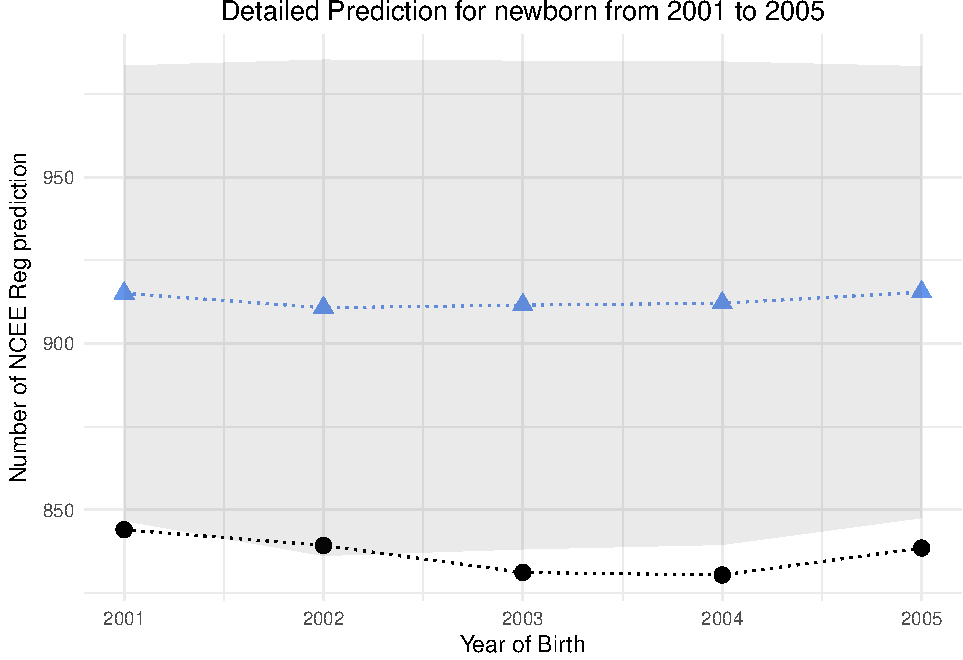
\includegraphics{NCEE_files/figure-latex/unnamed-chunk-6-2.pdf}

\begin{Shaded}
\begin{Highlighting}[]
\NormalTok{city.low <-}\StringTok{ }\KeywordTok{NCEE_function}\NormalTok{(NCEE_JHS,NCEE_reg)[[}\DecValTok{3}\NormalTok{]]}
\NormalTok{city.low.nu <-}\StringTok{ }\KeywordTok{as.vector}\NormalTok{(}\KeywordTok{t}\NormalTok{(city.low[,}\DecValTok{2}\OperatorTok{:}\DecValTok{32}\NormalTok{]))}
\NormalTok{city.fit <-}\StringTok{ }\KeywordTok{NCEE_function}\NormalTok{(NCEE_JHS,NCEE_reg)[[}\DecValTok{2}\NormalTok{]]}
\NormalTok{city.fit.nu <-}\StringTok{ }\KeywordTok{as.vector}\NormalTok{(}\KeywordTok{t}\NormalTok{(city.fit[,}\DecValTok{2}\OperatorTok{:}\DecValTok{32}\NormalTok{]))}
\NormalTok{city.high <-}\StringTok{ }\KeywordTok{NCEE_function}\NormalTok{(NCEE_JHS,NCEE_reg)[[}\DecValTok{4}\NormalTok{]]}
\NormalTok{city.high.nu <-}\StringTok{ }\KeywordTok{as.vector}\NormalTok{(}\KeywordTok{t}\NormalTok{(city.high[,}\DecValTok{2}\OperatorTok{:}\DecValTok{32}\NormalTok{]))}

\NormalTok{year_prd <-}\StringTok{ }\KeywordTok{c}\NormalTok{(}\KeywordTok{rep}\NormalTok{(}\StringTok{"23"}\NormalTok{,}\DecValTok{31}\NormalTok{),}\KeywordTok{rep}\NormalTok{(}\StringTok{"22"}\NormalTok{,}\DecValTok{31}\NormalTok{),}\KeywordTok{rep}\NormalTok{(}\StringTok{"21"}\NormalTok{,}\DecValTok{31}\NormalTok{),}\KeywordTok{rep}\NormalTok{(}\StringTok{"20"}\NormalTok{,}\DecValTok{31}\NormalTok{),}\KeywordTok{rep}\NormalTok{(}\StringTok{"19"}\NormalTok{,}\DecValTok{31}\NormalTok{))}

\NormalTok{pro_bind <-}\StringTok{ }\KeywordTok{data.frame}\NormalTok{(year_prd, }\DataTypeTok{province=}\KeywordTok{rep}\NormalTok{(province,}\DecValTok{5}\NormalTok{),city.low.nu,city.fit.nu,city.high.nu)}

\NormalTok{pl1 <-}\StringTok{ }
\NormalTok{pro_bind }\OperatorTok\StringTok{ }\KeywordTok{subset}\NormalTok{(province }\OperatorTok\StringTok{ }\KeywordTok{c}\NormalTok{(}\StringTok{"Beijing"}\NormalTok{, }\StringTok{"Tianjin"}\NormalTok{,}\StringTok{"Shanghai"}\NormalTok{, }\StringTok{"Hainan"}\NormalTok{)) }\OperatorTok
\KeywordTok{ggplot}\NormalTok{(}\KeywordTok{aes}\NormalTok{(year_prd, city.fit.nu, }\DataTypeTok{color=}\NormalTok{province)) }\OperatorTok{+}\StringTok{ }
\StringTok{  }\KeywordTok{geom_pointrange}\NormalTok{(}\KeywordTok{aes}\NormalTok{(}\DataTypeTok{ymin =}\NormalTok{ city.low.nu, }\DataTypeTok{ymax =}\NormalTok{ city.high.nu)) }\OperatorTok{+}
\StringTok{    }\KeywordTok{scale_color_manual}\NormalTok{(}\DataTypeTok{values=}\KeywordTok{wes_palette}\NormalTok{(}\StringTok{"Moonrise2"}\NormalTok{,}\DecValTok{4}\NormalTok{)) }\OperatorTok{+}
\StringTok{  }\KeywordTok{geom_line}\NormalTok{(}\KeywordTok{aes}\NormalTok{(}\DataTypeTok{group =}\NormalTok{ province)) }\OperatorTok{+}
\StringTok{  }\KeywordTok{theme_minimal}\NormalTok{() }\OperatorTok{+}
\StringTok{  }\KeywordTok{xlab}\NormalTok{(}\StringTok{"Year of Exam"}\NormalTok{) }\OperatorTok{+}
\StringTok{  }\KeywordTok{ylab}\NormalTok{(}\StringTok{"Number of Reg Prediction"}\NormalTok{) }\OperatorTok{+}
\StringTok{  }\KeywordTok{ggtitle}\NormalTok{(}\StringTok{"3 Metropolises & Hainan"}\NormalTok{) }\OperatorTok{+}
\StringTok{  }\KeywordTok{theme}\NormalTok{(}\DataTypeTok{plot.title =} \KeywordTok{element_text}\NormalTok{(}\DataTypeTok{hjust =} \FloatTok{0.5}\NormalTok{))}

\NormalTok{pl2 <-}
\NormalTok{pro_bind }\OperatorTok\StringTok{ }\KeywordTok{subset}\NormalTok{(province }\OperatorTok\StringTok{ }\KeywordTok{c}\NormalTok{(}\StringTok{"Qinghai"}\NormalTok{, }\StringTok{"Ningxia"}\NormalTok{,}\StringTok{"Xizang"}\NormalTok{, }\StringTok{"Xinjiang"}\NormalTok{)) }\OperatorTok
\KeywordTok{ggplot}\NormalTok{(}\KeywordTok{aes}\NormalTok{(year_prd, city.fit.nu, }\DataTypeTok{color=}\NormalTok{province)) }\OperatorTok{+}\StringTok{ }
\StringTok{  }\KeywordTok{geom_pointrange}\NormalTok{(}\KeywordTok{aes}\NormalTok{(}\DataTypeTok{ymin =}\NormalTok{ city.low.nu, }\DataTypeTok{ymax =}\NormalTok{ city.high.nu)) }\OperatorTok{+}
\StringTok{      }\KeywordTok{scale_color_manual}\NormalTok{(}\DataTypeTok{values=}\KeywordTok{wes_palette}\NormalTok{(}\StringTok{"Rushmore1"}\NormalTok{,}\DecValTok{4}\NormalTok{)) }\OperatorTok{+}
\StringTok{  }\KeywordTok{geom_line}\NormalTok{(}\KeywordTok{aes}\NormalTok{(}\DataTypeTok{group =}\NormalTok{ province)) }\OperatorTok{+}
\StringTok{  }\KeywordTok{theme_minimal}\NormalTok{() }\OperatorTok{+}
\StringTok{  }\KeywordTok{xlab}\NormalTok{(}\StringTok{"Year of Exam"}\NormalTok{) }\OperatorTok{+}
\StringTok{  }\KeywordTok{ylab}\NormalTok{(}\StringTok{"Number of Reg Prediction"}\NormalTok{) }\OperatorTok{+}
\StringTok{  }\KeywordTok{ggtitle}\NormalTok{(}\StringTok{"West 4 provinces"}\NormalTok{) }\OperatorTok{+}
\StringTok{  }\KeywordTok{theme}\NormalTok{(}\DataTypeTok{plot.title =} \KeywordTok{element_text}\NormalTok{(}\DataTypeTok{hjust =} \FloatTok{0.5}\NormalTok{))}

\NormalTok{pl3 <-}
\NormalTok{pro_bind }\OperatorTok\StringTok{ }\KeywordTok{subset}\NormalTok{(province }\OperatorTok\StringTok{ }\KeywordTok{c}\NormalTok{(}\StringTok{"Heilongjiang"}\NormalTok{, }\StringTok{"Jilin"}\NormalTok{,}\StringTok{"Liaoning"}\NormalTok{,}\StringTok{"Neimenggu"}\NormalTok{)) }\OperatorTok
\KeywordTok{ggplot}\NormalTok{(}\KeywordTok{aes}\NormalTok{(year_prd, city.fit.nu, }\DataTypeTok{color=}\NormalTok{province)) }\OperatorTok{+}\StringTok{ }
\StringTok{  }\KeywordTok{geom_pointrange}\NormalTok{(}\KeywordTok{aes}\NormalTok{(}\DataTypeTok{ymin =}\NormalTok{ city.low.nu, }\DataTypeTok{ymax =}\NormalTok{ city.high.nu)) }\OperatorTok{+}
\StringTok{      }\KeywordTok{scale_color_manual}\NormalTok{(}\DataTypeTok{values=}\KeywordTok{wes_palette}\NormalTok{(}\StringTok{"Zissou1"}\NormalTok{,}\DecValTok{4}\NormalTok{)) }\OperatorTok{+}
\StringTok{  }\KeywordTok{geom_line}\NormalTok{(}\KeywordTok{aes}\NormalTok{(}\DataTypeTok{group =}\NormalTok{ province)) }\OperatorTok{+}
\StringTok{  }\KeywordTok{theme_minimal}\NormalTok{() }\OperatorTok{+}
\StringTok{  }\KeywordTok{xlab}\NormalTok{(}\StringTok{"Year of Exam"}\NormalTok{) }\OperatorTok{+}
\StringTok{  }\KeywordTok{ylab}\NormalTok{(}\StringTok{"Number of Reg Prediction"}\NormalTok{) }\OperatorTok{+}
\StringTok{  }\KeywordTok{ggtitle}\NormalTok{(}\StringTok{"North-East 4 provinces"}\NormalTok{) }\OperatorTok{+}
\StringTok{  }\KeywordTok{theme}\NormalTok{(}\DataTypeTok{plot.title =} \KeywordTok{element_text}\NormalTok{(}\DataTypeTok{hjust =} \FloatTok{0.5}\NormalTok{))}

\NormalTok{pl4 <-}\StringTok{ }
\NormalTok{pro_bind }\OperatorTok\StringTok{ }\KeywordTok{subset}\NormalTok{(province }\OperatorTok\StringTok{ }\KeywordTok{c}\NormalTok{(}\StringTok{"Sichuan"}\NormalTok{, }\StringTok{"Guizhou"}\NormalTok{,}\StringTok{"Yunnan"}\NormalTok{,}\StringTok{"Guangxi"}\NormalTok{,}\StringTok{"Chongqing"}\NormalTok{)) }\OperatorTok
\KeywordTok{ggplot}\NormalTok{(}\KeywordTok{aes}\NormalTok{(year_prd, city.fit.nu, }\DataTypeTok{color=}\NormalTok{province)) }\OperatorTok{+}\StringTok{ }
\StringTok{  }\KeywordTok{geom_pointrange}\NormalTok{(}\KeywordTok{aes}\NormalTok{(}\DataTypeTok{ymin =}\NormalTok{ city.low.nu, }\DataTypeTok{ymax =}\NormalTok{ city.high.nu)) }\OperatorTok{+}
\StringTok{      }\KeywordTok{scale_color_manual}\NormalTok{(}\DataTypeTok{values=}\KeywordTok{wes_palette}\NormalTok{(}\StringTok{"Darjeeling1"}\NormalTok{,}\DecValTok{5}\NormalTok{)) }\OperatorTok{+}
\StringTok{  }\KeywordTok{geom_line}\NormalTok{(}\KeywordTok{aes}\NormalTok{(}\DataTypeTok{group =}\NormalTok{ province)) }\OperatorTok{+}
\StringTok{  }\KeywordTok{theme_minimal}\NormalTok{() }\OperatorTok{+}
\StringTok{  }\KeywordTok{xlab}\NormalTok{(}\StringTok{"Year of Exam"}\NormalTok{) }\OperatorTok{+}
\StringTok{  }\KeywordTok{ylab}\NormalTok{(}\StringTok{"Number of Reg Prediction"}\NormalTok{) }\OperatorTok{+}
\StringTok{  }\KeywordTok{ggtitle}\NormalTok{(}\StringTok{"South-West 5 provinces"}\NormalTok{) }\OperatorTok{+}
\StringTok{  }\KeywordTok{theme}\NormalTok{(}\DataTypeTok{plot.title =} \KeywordTok{element_text}\NormalTok{(}\DataTypeTok{hjust =} \FloatTok{0.5}\NormalTok{))}

\NormalTok{pl5 <-}
\NormalTok{pro_bind }\OperatorTok\StringTok{ }\KeywordTok{subset}\NormalTok{(province }\OperatorTok\StringTok{ }\KeywordTok{c}\NormalTok{(}\StringTok{"Zhejiang"}\NormalTok{, }\StringTok{"Jiangsu"}\NormalTok{,}\StringTok{"Anhui"}\NormalTok{)) }\OperatorTok
\KeywordTok{ggplot}\NormalTok{(}\KeywordTok{aes}\NormalTok{(year_prd, city.fit.nu, }\DataTypeTok{color=}\NormalTok{province)) }\OperatorTok{+}\StringTok{ }
\StringTok{  }\KeywordTok{geom_pointrange}\NormalTok{(}\KeywordTok{aes}\NormalTok{(}\DataTypeTok{ymin =}\NormalTok{ city.low.nu, }\DataTypeTok{ymax =}\NormalTok{ city.high.nu)) }\OperatorTok{+}
\StringTok{      }\KeywordTok{scale_color_manual}\NormalTok{(}\DataTypeTok{values=}\KeywordTok{wes_palette}\NormalTok{(}\StringTok{"FantasticFox1"}\NormalTok{,}\DecValTok{3}\NormalTok{)) }\OperatorTok{+}
\StringTok{  }\KeywordTok{geom_line}\NormalTok{(}\KeywordTok{aes}\NormalTok{(}\DataTypeTok{group =}\NormalTok{ province)) }\OperatorTok{+}
\StringTok{  }\KeywordTok{theme_minimal}\NormalTok{() }\OperatorTok{+}
\StringTok{  }\KeywordTok{xlab}\NormalTok{(}\StringTok{"Year of Exam"}\NormalTok{) }\OperatorTok{+}
\StringTok{  }\KeywordTok{ylab}\NormalTok{(}\StringTok{"Number of Reg Prediction"}\NormalTok{) }\OperatorTok{+}
\StringTok{  }\KeywordTok{ggtitle}\NormalTok{(}\StringTok{"South-East cost 3 provinces"}\NormalTok{) }\OperatorTok{+}
\StringTok{  }\KeywordTok{theme}\NormalTok{(}\DataTypeTok{plot.title =} \KeywordTok{element_text}\NormalTok{(}\DataTypeTok{hjust =} \FloatTok{0.5}\NormalTok{))}

\NormalTok{pl6 <-}
\NormalTok{pro_bind }\OperatorTok\StringTok{ }\KeywordTok{subset}\NormalTok{(province }\OperatorTok\StringTok{ }\KeywordTok{c}\NormalTok{(}\StringTok{"Guangdong"}\NormalTok{, }\StringTok{"Fujian"}\NormalTok{,}\StringTok{"Jiangxi"}\NormalTok{)) }\OperatorTok
\KeywordTok{ggplot}\NormalTok{(}\KeywordTok{aes}\NormalTok{(year_prd, city.fit.nu, }\DataTypeTok{color=}\NormalTok{province)) }\OperatorTok{+}\StringTok{ }
\StringTok{  }\KeywordTok{geom_pointrange}\NormalTok{(}\KeywordTok{aes}\NormalTok{(}\DataTypeTok{ymin =}\NormalTok{ city.low.nu, }\DataTypeTok{ymax =}\NormalTok{ city.high.nu)) }\OperatorTok{+}
\StringTok{      }\KeywordTok{scale_color_manual}\NormalTok{(}\DataTypeTok{values=}\KeywordTok{wes_palette}\NormalTok{(}\StringTok{"GrandBudapest1"}\NormalTok{,}\DecValTok{3}\NormalTok{)) }\OperatorTok{+}
\StringTok{  }\KeywordTok{geom_line}\NormalTok{(}\KeywordTok{aes}\NormalTok{(}\DataTypeTok{group =}\NormalTok{ province)) }\OperatorTok{+}
\StringTok{  }\KeywordTok{theme_minimal}\NormalTok{() }\OperatorTok{+}
\StringTok{  }\KeywordTok{xlab}\NormalTok{(}\StringTok{"Year of Exam"}\NormalTok{) }\OperatorTok{+}
\StringTok{  }\KeywordTok{ylab}\NormalTok{(}\StringTok{"Number of Reg Prediction"}\NormalTok{) }\OperatorTok{+}
\StringTok{  }\KeywordTok{ggtitle}\NormalTok{(}\StringTok{"South-Coast 3 provinces"}\NormalTok{) }\OperatorTok{+}
\StringTok{  }\KeywordTok{theme}\NormalTok{(}\DataTypeTok{plot.title =} \KeywordTok{element_text}\NormalTok{(}\DataTypeTok{hjust =} \FloatTok{0.5}\NormalTok{))}

\NormalTok{pl7 <-}
\NormalTok{pro_bind }\OperatorTok\StringTok{ }\KeywordTok{subset}\NormalTok{(province }\OperatorTok\StringTok{ }\KeywordTok{c}\NormalTok{(}\StringTok{"Hunan"}\NormalTok{, }\StringTok{"Hubei"}\NormalTok{,}\StringTok{"Henan"}\NormalTok{,}\StringTok{"Shandong"}\NormalTok{)) }\OperatorTok
\KeywordTok{ggplot}\NormalTok{(}\KeywordTok{aes}\NormalTok{(year_prd, city.fit.nu, }\DataTypeTok{color=}\NormalTok{province)) }\OperatorTok{+}\StringTok{ }
\StringTok{  }\KeywordTok{geom_pointrange}\NormalTok{(}\KeywordTok{aes}\NormalTok{(}\DataTypeTok{ymin =}\NormalTok{ city.low.nu, }\DataTypeTok{ymax =}\NormalTok{ city.high.nu)) }\OperatorTok{+}
\StringTok{      }\KeywordTok{scale_color_manual}\NormalTok{(}\DataTypeTok{values=}\KeywordTok{wes_palette}\NormalTok{(}\StringTok{"Cavalcanti1"}\NormalTok{,}\DecValTok{4}\NormalTok{)) }\OperatorTok{+}
\StringTok{  }\KeywordTok{geom_line}\NormalTok{(}\KeywordTok{aes}\NormalTok{(}\DataTypeTok{group =}\NormalTok{ province)) }\OperatorTok{+}
\StringTok{  }\KeywordTok{theme_minimal}\NormalTok{() }\OperatorTok{+}
\StringTok{  }\KeywordTok{xlab}\NormalTok{(}\StringTok{"Year of Exam"}\NormalTok{) }\OperatorTok{+}
\StringTok{  }\KeywordTok{ylab}\NormalTok{(}\StringTok{"Number of Reg Prediction"}\NormalTok{) }\OperatorTok{+}
\StringTok{  }\KeywordTok{ggtitle}\NormalTok{(}\StringTok{"North-Central 4 provinces"}\NormalTok{) }\OperatorTok{+}
\StringTok{  }\KeywordTok{theme}\NormalTok{(}\DataTypeTok{plot.title =} \KeywordTok{element_text}\NormalTok{(}\DataTypeTok{hjust =} \FloatTok{0.5}\NormalTok{))}

\NormalTok{pl8 <-}
\NormalTok{pro_bind }\OperatorTok\StringTok{ }\KeywordTok{subset}\NormalTok{(province }\OperatorTok\StringTok{ }\KeywordTok{c}\NormalTok{(}\StringTok{"Shanxi"}\NormalTok{, }\StringTok{"Shaanxi"}\NormalTok{,}\StringTok{"Hebei"}\NormalTok{,}\StringTok{"Gansu"}\NormalTok{)) }\OperatorTok
\KeywordTok{ggplot}\NormalTok{(}\KeywordTok{aes}\NormalTok{(year_prd, city.fit.nu, }\DataTypeTok{color=}\NormalTok{province)) }\OperatorTok{+}\StringTok{ }
\StringTok{  }\KeywordTok{geom_pointrange}\NormalTok{(}\KeywordTok{aes}\NormalTok{(}\DataTypeTok{ymin =}\NormalTok{ city.low.nu, }\DataTypeTok{ymax =}\NormalTok{ city.high.nu)) }\OperatorTok{+}
\StringTok{      }\KeywordTok{scale_color_manual}\NormalTok{(}\DataTypeTok{values=}\KeywordTok{wes_palette}\NormalTok{(}\StringTok{"Rushmore"}\NormalTok{,}\DecValTok{4}\NormalTok{)) }\OperatorTok{+}
\StringTok{  }\KeywordTok{geom_line}\NormalTok{(}\KeywordTok{aes}\NormalTok{(}\DataTypeTok{group =}\NormalTok{ province)) }\OperatorTok{+}
\StringTok{  }\KeywordTok{theme_minimal}\NormalTok{() }\OperatorTok{+}
\StringTok{  }\KeywordTok{xlab}\NormalTok{(}\StringTok{"Year of Exam"}\NormalTok{) }\OperatorTok{+}
\StringTok{  }\KeywordTok{ylab}\NormalTok{(}\StringTok{"Number of Reg Prediction"}\NormalTok{) }\OperatorTok{+}
\StringTok{  }\KeywordTok{ggtitle}\NormalTok{(}\StringTok{"West-Central 4 provinces"}\NormalTok{) }\OperatorTok{+}
\StringTok{  }\KeywordTok{theme}\NormalTok{(}\DataTypeTok{plot.title =} \KeywordTok{element_text}\NormalTok{(}\DataTypeTok{hjust =} \FloatTok{0.5}\NormalTok{))}

\CommentTok{# =====Display===== #}

\KeywordTok{grid.arrange}\NormalTok{(pl1, pl2, pl3, pl4, }\DataTypeTok{nrow =} \DecValTok{2}\NormalTok{)}
\end{Highlighting}
\end{Shaded}

\includegraphics{NCEE_files/figure-latex/unnamed-chunk-7-1.pdf}

\begin{Shaded}
\begin{Highlighting}[]
\KeywordTok{grid.arrange}\NormalTok{(pl5, pl6, pl7, pl8, }\DataTypeTok{nrow =} \DecValTok{2}\NormalTok{)}
\end{Highlighting}
\end{Shaded}

\includegraphics{NCEE_files/figure-latex/unnamed-chunk-7-2.pdf}


\end{document}
